% ======================================================================
% Přednáška 1 (OneNote: \uv{1. Prednaska, 2.cast}, 3. 10. 2022)
% Rozptyl tvrdých koulí, Rutherfordův rozptyl – klasické odvození (začátek)
% ======================================================================
\section{Účinný průřez: tvrdé koule a Rutherfordův rozptyl}

\strana{P01-1}
Celá jaderná a částicová fyzika stojí na jednom experimentálním postupu: \emph{něco na něco pošleme a díváme se, kam to odletí}. Veličina, která převádí \uv{kolik částic odletělo kam} na vlastnost samotné interakce (nezávislou na tom, jak silný svazek jsme použili a jak tlustý terč), je \kw{účinný průřez}. Než se pustíme do skutečných jader, ukážeme si celý postup na nejjednodušším možném modelu -- na srážce dvou \kw{tvrdých koulí}. Tam je všechno čistě geometrické, a proto je dobře vidět, \emph{co} účinný průřez znamená. Potom stejný postup zopakujeme pro coulombovskou sílu, čímž dostaneme slavný Rutherfordův vzorec, na kterém byl objeveno atomové jádro.

\subsection{Rozptyl tvrdé koule na tvrdé kouli}

Uvažujme malou kouli o poloměru $r_2$ (projektil, hmotnost $m_2$), která letí rovnoběžně s osou a míjí velkou kouli o poloměru $r_1$ (terč, hmotnost $m_1$). Kolmá vzdálenost přímky, po které projektil přilétá, od středu terče se nazývá \kw{srážkový (záměrný) parametr} $b$. Nejprve předpokládáme $m_1 \gg m_2$, takže terč se při srážce nepohne (laboratorní soustava = soustava terče).

\begin{center}
\begin{tikzpicture}[scale=1.0]
  % osa terče a dráha projektilu
  \draw[dashed] (-4.2,0) -- (3.2,0);
  \draw[dashed] (-4.2,1.6) -- (0.0,1.6);
  \draw[dashed] (0.0,1.6) -- (3.2,1.6);
  % terč
  \draw[thick] (0,0) circle (1.25);
  \fill (0,0) circle (0.04);
  \draw[->] (0,0) -- ({1.25*cos(60)},{1.25*sin(60)}) node[midway,right=1pt] {\small $r_1$};
  % projektil v okamžiku dotyku: střed ve vzdálenosti r1+r2 od středu terče
  \coordinate (P) at ({1.85*cos(120)},{1.85*sin(120)});
  \draw[thick] (P) circle (0.6);
  \fill (P) circle (0.04);
  \draw[->] (P) -- ++(100:0.6) node[above left=-2pt] {\small $r_2$};
  % spojnice středů (normála dotyku)
  \draw[gray] (0,0) -- (P);
  % odražený směr: zrcadlení podle normály -> směr pod úhlem theta = 180-2*60 = 60 st.
  \draw[->,thick] (P) -- ++(60:2.4);
  \draw (P) ++(0.9,0) arc (0:60:0.9);
  \node at ($(P)+(30:1.2)$) {$\theta$};
  % b
  \draw[<->] (-3.8,0) -- (-3.8,1.6) node[midway,left] {$b$};
  \node[right] at (3.3,0.8) {$m_1 \gg m_2$};
\end{tikzpicture}
\end{center}

Projektil se od koule odrazí jako od zrcadla: úhel dopadu na tečnou rovinu v bodě dotyku je roven úhlu odrazu. Spojnice středů v okamžiku dotyku má délku $r_1+r_2$ a svírá se směrem dopadu úhel, jehož doplněk do $\pi$ je rozdělen symetricky. Elementární geometrie dává vztah mezi záměrným parametrem a \kw{úhlem rozptylu} $\theta$:
\begin{equation}
  b = (r_1+r_2)\cos\frac{\theta}{2}.
\end{equation}
Čelní srážka ($b=0$) dává $\theta=\pi$ (odraz zpět), tečné míjení ($b=r_1+r_2$) dává $\theta=0$. Celá informace o \uv{síle} je tady zakódována v tom, jak $b$ závisí na $\theta$; přesně tuto závislost budeme za chvíli hledat i pro Coulombovu sílu.

\paragraph{Definice účinného průřezu.}
Pošleme na terč homogenní svazek s \kw{hustotou toku} $j$ (počet částic za jednotku času prošlých jednotkovou plochou kolmou ke svazku). Projektily se záměrným parametrem v intervalu $(b, b+\dd b)$ prolétají mezikružím o ploše
\[
  S = 2\pi b\,\dd b ,
\]
a všechny se rozptýlí do úhlů v intervalu $(\theta,\theta+\dd\theta)$.

\begin{center}
\begin{tikzpicture}[scale=1.0]
  \fill[pattern=north east lines,pattern color=red!60] (0,0) circle (1.45);
  \fill[white] (0,0) circle (1.2);
  \draw[thick] (0,0) circle (1.2);
  \draw[thick] (0,0) circle (1.45);
  \fill (0,0) circle (0.035);
  \draw[->] (0,0) -- (0,1.2) node[midway,right] {$b$};
  \draw[red,thick] (1.2*0.8,1.2*0.6) -- (1.45*0.8,1.45*0.6);
  \node[red] at (1.65,1.15) {$\dd b$};
  \node[right] at (2.0,0) {$S = 2\pi b\,\dd b$};
\end{tikzpicture}
\end{center}

Počet rozptýlených částic za jednotku času je $j\cdot 2\pi b\,\dd b$. Abychom dostali veličinu, která nezávisí na intenzitě svazku, vydělíme ho hustotou toku -- tím dostaneme \emph{plochu}:
\begin{equation}
  \dd\sigma = \frac{j\, 2\pi b\, \dd b}{j} = 2\pi b\,\dd b .
\end{equation}

\begin{definice}[Účinný průřez]
\kw{Diferenciální účinný průřez} $\dv*{\sigma}{\Omega}$ je počet částic rozptýlených za jednotku času do prostorového úhlu $\dd\Omega$ kolem směru $(\theta,\varphi)$, dělený hustotou toku dopadajících částic a velikostí $\dd\Omega$. \kw{Celkový účinný průřez} je jeho integrál přes všechny směry, $\sigma = \int \dv*{\sigma}{\Omega}\,\dd\Omega$. Má rozměr plochy -- je to \uv{efektivní terčová plocha}, kterou terč staví do cesty svazku.
\end{definice}

Prostorový úhel odpovídající pásu úhlů $(\theta,\theta+\dd\theta)$ (po integraci přes azimut, kvůli osové symetrii) je $\dd\Omega = 2\pi\sin\theta\,\dd\theta$. Dosadíme $b(\theta)$ a $\dd b = (r_1+r_2)\,(-\sin\tfrac{\theta}{2})\tfrac{\dd\theta}{2}$:
\begin{equation}
  \dv{\sigma}{\Omega} = \frac{2\pi b\,\dd b}{2\pi\sin\theta\,\dd\theta}
  = \frac{(r_1+r_2)^2 \cos\frac{\theta}{2}\,\sin\frac{\theta}{2}\,(-1)\,\frac{\dd\theta}{2}}{\sin\theta\,\dd\theta}.
\end{equation}
Znaménko minus jen říká, že s rostoucím $b$ klesá $\theta$; účinný průřez bereme v absolutní hodnotě. S využitím $\sin\theta = 2\sin\frac{\theta}{2}\cos\frac{\theta}{2}$ se vše pokrátí:
\begin{equation}
  \vzorec{\dv{\sigma}{\Omega} = \frac14 (r_1+r_2)^2}
\end{equation}
Rozptyl tvrdých koulí (s nepohyblivým terčem) je tedy \kw{izotropní} -- do každého prostorového úhlu letí stejně částic. Celkový účinný průřez je
\begin{equation}
  \sigma = \int \dv{\sigma}{\Omega}\,\dd\Omega = \frac14 (r_1+r_2)^2\, 4\pi = \pi (r_1+r_2)^2 ,
\end{equation}
což je přesně geometrická plocha kruhu o poloměru $r_1+r_2$: projektil se rozptýlí právě tehdy, když jeho střed proletí uvnitř tohoto kruhu. Tento výsledek je dobrou kontrolou, že definice účinného průřezu dává intuitivně správnou \uv{terčovou plochu}.

\begin{vysvetleni}[Proč se zajímáme o $\dv*{\sigma}{\Omega}$, a ne jen o $\sigma$]
Celkový účinný průřez nám řekne jen \uv{jak velký} terč je. Úhlové rozdělení $\dv*{\sigma}{\Omega}$ ale nese informaci o \emph{tvaru} interakce: izotropní rozdělení znamená tvrdou kouli, $\sin^{-4}(\theta/2)$ znamená bodový coulombovský náboj (viz níže), odchylky od něj znamenají, že náboj je rozmazaný (formfaktor, viz přednáška 2). Celá historie odhalování struktury hmoty -- jádro (Rutherford 1911), velikost jader (Hofstadter), kvarky v protonu (hluboce nepružný rozptyl) -- je historií měření $\dv*{\sigma}{\Omega}$. Střední volná dráha v terči s koncentrací $n$ rozptylových center je pak $\lambda = 1/(n\sigma)$ (viz Davídkovy slajdy, \uv{Účinný průřez $\sigma$}).
\end{vysvetleni}

\subsection{Srovnatelné hmotnosti: přechod do těžišťové soustavy}

Pokud \pozor{neplatí $m_1 \gg m_2$}, terč při srážce získá zpětný ráz a jednoduchá geometrie výše přestane platit. Standardní postup je \kw{přejít do těžišťové soustavy} (CMS): v ní mají obě koule opačné hybnosti stejné velikosti, srážka je opět \uv{zrcadlový odraz} a účinný průřez v těžišťových úhlech je opět izotropní, $\dv*{\sigma}{\Omega_{\mathrm{cm}}} = \frac14(r_1+r_2)^2$. Do laboratoře se pak vrátíme transformací úhlů (a tedy i prostorových úhlů) -- právě Jakobián této transformace způsobí, že laboratorní rozdělení už izotropní není.

\begin{center}
\begin{tikzpicture}[scale=1.0]
  \draw (-3,0.25) -- (-0.25,0.25);
  \draw (0,0.25) circle (0.25);
  \draw (0,-0.25) circle (0.25);
  \draw (0.25,-0.25) -- (2.0,-0.25);
  \draw[->,thick] (0.2,0.4) -- (1.8,1.7);
  \draw[->,thick] (-0.15,-0.45) -- (-1.2,-1.4);
\end{tikzpicture}
\end{center}

\strana{P01-2}
Výsledek transformace do laboratorní soustavy (úhel $\theta$ je laboratorní úhel rozptylu projektilu) je
\begin{equation}
  \dv{\sigma}{\Omega} = \frac{(r_1+r_2)^2}{4}\left\{ 2\,\oprava{\frac{m_2}{m_1}}{\frac{m_1}{m_2}}\cos\theta + \frac{1+\left(\frac{m_2}{m_1}\right)^2\cos 2\theta}{\sqrt{1-\left(\frac{m_2}{m_1}\right)^2\sin^2\theta}}\right\}
  \qquad\text{pro } m_2 \le m_1 .
\end{equation}
\pozor{Pozor na poměr hmotností:} ve vzorci vystupuje poměr \emph{hmotnosti projektilu ku hmotnosti terče}. Při značení z obrázku výše (terč $m_1$, projektil $m_2$) je to $m_2/m_1$; v poznámkách je ve všech třech místech napsáno $m_1/m_2$, což s podmínkou $m_2\le m_1$ nesouhlasí (odmocnina by pro $m_1>m_2$ a velké úhly byla imaginární). Kontrola: pro $m_2/m_1\to 0$ přejde závorka v $\{0 + 1\} = 1$ a dostaneme izotropní výsledek $\frac14(r_1+r_2)^2$ z předchozí části, jak má být.

\paragraph{Speciálně pro $m_1 = m_2$} (např. srážka dvou stejných koulí kulečníku, nebo neutron na protonu):
\begin{equation}
  \dv{\sigma}{\Omega} = \frac{(r_1+r_2)^2}{4}\left\{2\cos\theta + \frac{1+\cos 2\theta}{\sqrt{1-\sin^2\theta}}\right\}
  = \frac{(r_1+r_2)^2}{4}\left\{2\cos\theta + \frac{2\cos^2\theta}{\cos\theta}\right\}
  = (r_1+r_2)^2\cos\theta ,
\end{equation}
kde jsme použili $1+\cos2\theta = 2\cos^2\theta$ a $\sqrt{1-\sin^2\theta} = \cos\theta$ (pro $\theta<\pi/2$). Rozdělení je úměrné $\cos\theta$ a pro $\theta \ge \pi/2$ je nulové: koule stejné hmotnosti se nikdy neodrazí dozadu -- v nejlepším případě (čelní srážka) se projektil zastaví a veškerou hybnost předá terči. Integrál přes horní polokouli dává opět $\int_0^{\pi/2}(r_1+r_2)^2\cos\theta\,2\pi\sin\theta\,\dd\theta = \pi(r_1+r_2)^2$ -- celkový průřez na soustavě nezávisí, mění se jen úhlové rozdělení.

\paragraph{Obrácený případ} $m_2 > m_1$ (těžký projektil na lehkém terči):
\begin{equation}
  \dv{\sigma}{\Omega} = \frac{(r_1+r_2)^2}{2}\,
  \frac{1+\oprava{\left(\frac{m_2}{m_1}\right)^2}{\frac{m_1}{m_2}}\cos 2\theta}{\sqrt{1-\left(\frac{m_2}{m_1}\right)^2\sin^2\theta}} .
\end{equation}
Tady se těžký projektil může v laboratoři odchýlit nejvýše o úhel $\theta_{\max} = \arcsin(m_1/m_2)$ (pro větší úhly je odmocnina imaginární) a do každého laboratorního úhlu $\theta<\theta_{\max}$ vedou \emph{dva} různé těžišťové úhly. Jejich příspěvky se sečtou: členy $\pm 2\gamma\cos\theta$ (kde $\gamma = m_2/m_1$) se vyruší a zbude dvojnásobek druhého členu -- odtud prefaktor $\frac12$ místo $\frac14$. Ve shodě s předchozím vzorcem i zde vystupuje poměr projektil/terč, $m_2/m_1$, a v čitateli musí být jeho \emph{druhá mocnina} (v poznámkách $\frac{m_1}{m_2}$ bez kvadrátu, ve jmenovateli $\frac{m_1}{m_2}$).

\begin{vysvetleni}[Odkud se laboratorní vzorce berou]
Označme $\gamma = m_{\text{proj}}/m_{\text{terč}}$. Pro úhel rozptylu v laboratoři $\theta$ a v těžišťové soustavě $\theta_c$ platí $\tan\theta = \frac{\sin\theta_c}{\gamma + \cos\theta_c}$ a
\[
  \dv{\sigma}{\Omega} = \dv{\sigma}{\Omega_c}\,\left|\dv{\Omega_c}{\Omega}\right|,
  \qquad
  \dv{\Omega_c}{\Omega} = \frac{(1+\gamma^2+2\gamma\cos\theta_c)^{3/2}}{|1+\gamma\cos\theta_c|}
  = \frac{\left(\gamma\cos\theta \pm \sqrt{1-\gamma^2\sin^2\theta}\right)^2}{\sqrt{1-\gamma^2\sin^2\theta}} .
\]
Pro $\gamma<1$ přispívá jen znaménko $+$ a s $\dv*{\sigma}{\Omega_c} = \frac14(r_1+r_2)^2$ dostaneme první vzorec. Pro $\gamma>1$ přispívají obě větve, $(\gamma\cos\theta+s)^2 + (\gamma\cos\theta-s)^2 = 2(1+\gamma^2\cos2\theta)$, a vyjde vzorec pro obrácený případ. Pro $\gamma=1$ splynou oba vzorce v $(r_1+r_2)^2\cos\theta$.
\end{vysvetleni}

\subsection{Rutherfordův experiment}

Teď stejný postup použijeme na situaci, kvůli které byl celý aparát vymyšlen. Rutherford, Geiger a Marsden (1909--1911) ostřelovali tenkou zlatou (a stříbrnou) fólii částicemi $\alpha$ z radonového zářiče a pozorovali scintilace na stínítku ze ZnS pod úhly $5^\circ$ až $150^\circ$ (viz Davídkovy slajdy, \uv{Rutherfordův experiment (1), (2)}). Podle Thomsonova modelu (\uv{pudink s rozinkami}) měly být odchylky nepatrné; pozorovaný počet částic rozptýlených pod velkými úhly byl ale o mnoho řádů vyšší. Abychom pochopili proč, spočteme, jaké úhlové rozdělení dává rozptyl bodového náboje na \emph{bodovém} náboji.

\begin{center}
\begin{tikzpicture}[scale=1.0]
  % jádro
  \fill (0,0) circle (0.1) node[below right] {$Qe$};
  % osa a dráha přilétající částice
  \draw[dashed] (-5,0) -- (3,0);
  \draw[dashed] (-5,0.6) -- (2.4,0.6);
  \fill (-4.6,0.6) circle (0.05) node[above] {$qe$};
  % hyperbola: rovnoběžná s osou na začátku, odkloní se o theta
  \draw[thick,->] plot[smooth] coordinates {(-4.6,0.6) (-2.5,0.65) (-1.2,0.8) (-0.2,1.15) (0.6,1.7) (1.3,2.5) (1.8,3.2)};
  % asymptota výletu
  \draw[dashed] (-0.9,-0.6) -- (2.0,3.3);
  \draw (1.1,0.6) arc (0:53:0.9);
  \node at (1.25,1.05) {$\theta$};
  \draw[<->] (-5.2,0) -- (-5.2,0.6) node[midway,left] {$b$};
\end{tikzpicture}
\end{center}

Částice s nábojem $qe$ (pro $\alpha$: $q=2$) přilétá rychlostí $v_0$ se záměrným parametrem $b$ k jádru s nábojem $Qe$ (pro zlato $Q=79$), které považujeme za nepohyblivé ($m_{\text{Au}}\gg m_\alpha$). Působí na ni odpudivá Coulombova síla
\begin{equation}
  F = \frac{1}{4\pi\varepsilon_0}\,\frac{qQe^2}{r^2},
\end{equation}
kde $r$ je okamžitá vzdálenost od jádra. Dráha je hyperbola, ale tu nebudeme potřebovat celou -- stačí nám spočítat \emph{celkovou změnu hybnosti}
\begin{equation}
  \Delta\vec{p} = \int \vec{F}\,\dd t ,
\end{equation}
protože z ní plyne úhel rozptylu.

\paragraph{Geometrie hybností.}
Coulombova síla je konzervativní a jádro je nepohyblivé, takže velikost hybnosti se nemění: $|\vec p_{\mathrm{in}}| = |\vec p_{\mathrm{out}}| = p = m v_0$. Vektory $\vec p_{\mathrm{in}}$, $\vec p_{\mathrm{out}}$ a $\Delta\vec p = \vec p_{\mathrm{out}}-\vec p_{\mathrm{in}}$ tvoří rovnoramenný trojúhelník s úhlem $\theta$ u vrcholu:

\begin{center}
\begin{tikzpicture}[scale=1.0]
  \coordinate (A) at (0,0);
  \coordinate (B) at (3,0);
  \coordinate (C) at ({3*cos(40)},{3*sin(40)});
  \fill[cyan!25] (A) -- (B) -- ($(B)!0.5!(C)$) -- cycle;
  \draw[->,thick] (A) -- (B) node[midway,below] {$\vec p_{\mathrm{in}}$};
  \draw[->,thick] (A) -- (C) node[midway,above left] {$\vec p_{\mathrm{out}}$};
  \draw[->,thick,red] (B) -- (C) node[midway,right] {$\Delta\vec p$};
  \draw[dotted] (A) -- ($(B)!0.5!(C)$);
  \draw (0.9,0) arc (0:20:0.9) node[pos=0.6,right] {\small $\frac{\theta}{2}$};
  \draw (1.5,0) arc (0:40:1.5);
  \node at (1.75,0.7) {$\theta$};
\end{tikzpicture}
\end{center}

Polovina trojúhelníku (podle osy úhlu $\theta$) je pravoúhlý trojúhelník s přeponou $p$ a protilehlou odvěsnou $\Delta p/2$:
\begin{equation}
  \sin\frac{\theta}{2} = \frac{\Delta p}{2p} \quad\Longrightarrow\quad \Delta p = 2p\sin\frac{\theta}{2}.
\end{equation}

\paragraph{Výpočet impulzu síly.}
Ze symetrie hyperboly (je souměrná podle přímky spojující jádro s vrcholem dráhy) míří $\Delta\vec p$ podél této osy symetrie; složky síly kolmé na ni se mezi příletem a odletem vyruší. Zavedeme proto polární úhel $\varphi$ polohy částice měřený \emph{od osy symetrie} (tj. od směru $\Delta\vec p$).

\begin{center}
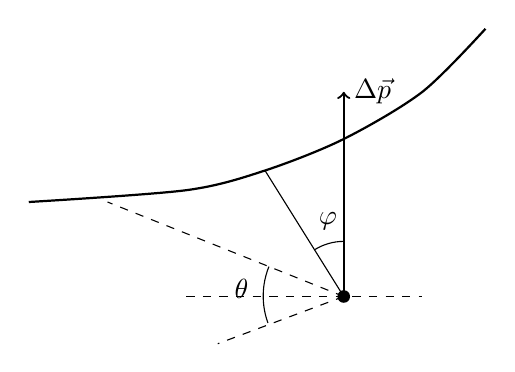
\begin{tikzpicture}[scale=1.0]
  \fill (0,0) circle (0.08);
  % dráha souměrná podle svislé osy
  \draw[thick] plot[smooth] coordinates {(-4,1.2) (-2,1.35) (-1,1.6) (0,2.0) (1,2.6) (1.8,3.4)};
  \draw[->,thick] (0,0) -- (0,2.6) node[right] {$\Delta\vec p$};
  \draw (0,0) -- (-1,1.6);
  \draw (0,0.7) arc (90:122:0.7);
  \node at (-0.2,0.95) {$\varphi$};
  \draw[dashed] (0,0) -- (-1.6,-0.6);
  \draw[dashed] (0,0) -- (-3,1.2);
  \draw (-0.95,0.38) arc (158:200:1.0);
  \node at (-1.3,0.1) {$\theta$};
  \draw[dashed] (-2.0,0) -- (1.0,0);
\end{tikzpicture}
\end{center}

Na začátku (daleko vlevo) a na konci (daleko vpravo nahoře) má poloha částice úhel
\begin{align}
  \varphi(t=-\infty) &= -\frac{\pi-\theta}{2} \qquad\text{na začátku},\\
  \varphi(t=+\infty) &= +\frac{\pi-\theta}{2} \qquad\text{na konci}.
\end{align}
(Celkem se směr průvodiče otočí o $\pi-\theta$: bez rozptylu by to bylo $\pi$, rozptyl o $\theta$ tuto otočku zkrátí.)
Do $\Delta p$ přispívá jen průmět síly do směru osy, tedy $F\cos\varphi$. Integrál přes čas převedeme na integrál přes úhel substitucí $\dd t = \dd\varphi / |\dv*{\varphi}{t}|$:
\begin{equation}
  \Delta p = 2p\sin\frac{\theta}{2} = \int_{-\infty}^{\infty}\dd t\, F\cos\varphi
  = \int_{-\frac{\pi-\theta}{2}}^{+\frac{\pi-\theta}{2}} \dd\varphi\, \frac{1}{\left|\dv{\varphi}{t}\right|}\, F(\varphi)\cos\varphi = (*)
\end{equation}

\strana{P01-3}
Úhlovou rychlost $\dv*{\varphi}{t}=\omega$ určíme ze \kw{zákona zachování momentu hybnosti} (síla je centrální). Daleko od jádra je moment hybnosti $l = m v_0 b$ (rychlost krát \uv{rameno} $b$), během pohybu $l = m\omega r^2$:
\begin{equation}
  \dv{\varphi}{t} = \omega ;\qquad l = m\omega r^2 = m v_0 b = \text{konst.}
  \quad\Longrightarrow\quad \omega = \frac{v_0 b}{r^2}.
\end{equation}
Tohle je klíčový trik celého odvození: neznámou závislost $r(\varphi)$ (tvar hyperboly) nepotřebujeme, protože $1/\omega$ obsahuje $r^2$ a síla $1/r^2$ -- obojí se pokrátí. Dosazením dostaneme
\begin{equation}
  (*)\qquad 2p\sin\frac{\theta}{2} = \int_{-\frac{\pi-\theta}{2}}^{\frac{\pi-\theta}{2}}
  \underbrace{\frac{qQe^2}{4\pi\varepsilon_0}\,\frac{1}{r^2(\varphi)}}_{F(\varphi)}\,\cos\varphi\;\frac{r^2(\varphi)}{v_0 b}\,\dd\varphi .
\end{equation}
Integrál se dopočítá v následující přednášce.
